\documentclass[12pt]{article}
\usepackage[english]{babel}
\usepackage[utf8x]{inputenc}
\usepackage{amsmath}
\usepackage{graphicx}
\usepackage[a4paper]{geometry}

\begin{document}
\begin{titlepage}

% definition of custom command for horizontal lines
\newcommand{\HRule}{\rule{\linewidth}{0.5mm}}

\center
% HEADING
\textsc{\LARGE University of Dublin,\\Trinity College}\\[1.0cm]

\includegraphics[width=0.2\textwidth]{logo.png}

\HRule \\[0.4cm]
\textsc{\Large JS Engineering: 3C2 Digital Circuits}\\[0.25cm]
\textsc{\large D1: The Bipolar Junction Transistor Inverter}\\[0.1cm]
\HRule \\[0.4cm]
 
% AUTHORS
\begin{minipage}{0.5\textwidth}
\begin{flushleft} \large
\emph{Author:}
\\Edmond \textsc{O'Flynn} 12304742
\end{flushleft}
\end{minipage}
~
\begin{minipage}{0.4\textwidth}
\begin{flushleft} 
\large
\emph{Demonstrator:} \\
Cormac \textsc{Molloy} 
\end{flushleft}
\end{minipage}\\[3cm]

% DATE
{\large \today}\\[2cm] 

% LOGO
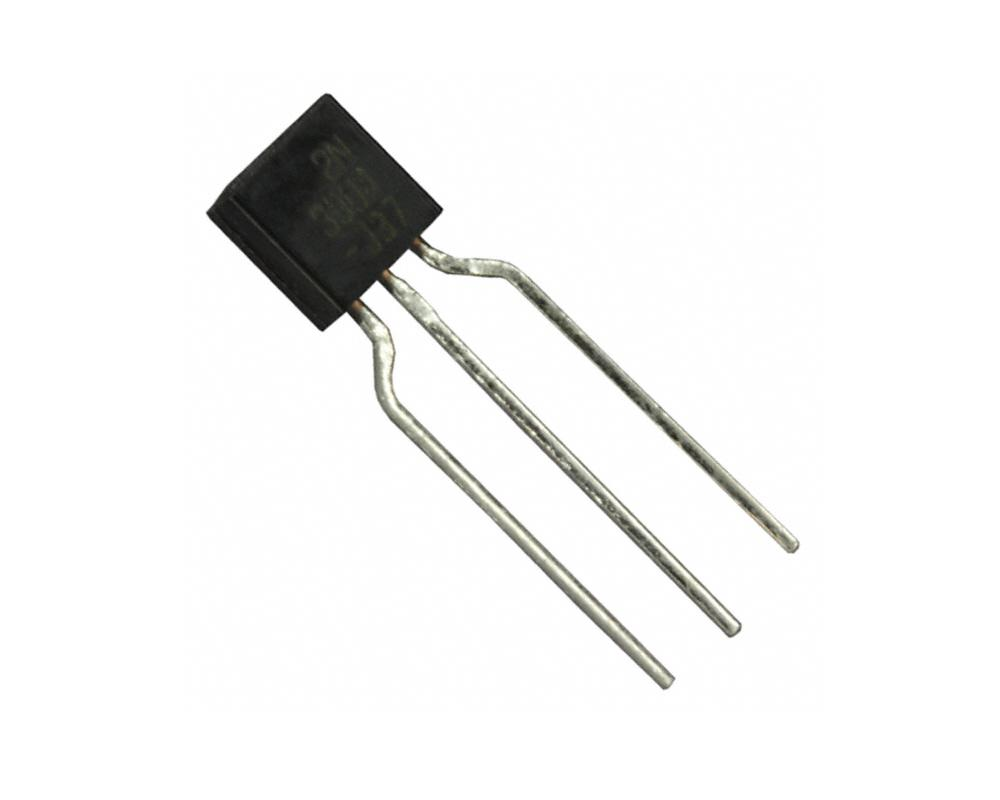
\includegraphics[width=0.4\textwidth]{bjt.JPG}
\clearpage
\end{titlepage}

\newgeometry{top=1cm,left=1cm,bottom=2cm,right=1cm}
\tableofcontents
\addcontentsline{toc}{section}{References}
\thispagestyle{empty}
\cleardoublepage
\setcounter{page}{1}

\newgeometry{top=2cm,left=2cm,bottom=2cm,right=2cm}

\section{Abstract}
Lab D1 introduces the concept of circuitry simulation in the MultiSim 13.0 environment, and theory associated with the Bipolar Junction Transistor within various characteristics spanning current-voltage, transfer characteristics, and dynamic properties within the inverter itself.
\section{BJT Current - Voltage Characteristics}
\subsection{Theory}
\subsubsection{What is a Bipolar Junction Transistor?}
Transistors are a fundamental part of electronics in the modern day. They may act as switches, control digital information, as well as within amplifiers. BJTs are generally used for small loads typically less than 1 amp of current. 

A \emph{Bipolar Junction Transistor} is a transistor that is subject to both hole and charge carriers under two types of manufacture: \emph{NPN} and \emph{PNP}. A BJT pertains to that of providing a means of gain in current amplification which allows the component to be used in integrated circuits as either a switch or amplifier, therefore giving it a large range of uses in electronic equipment.

There are three regions within a BJT: \emph{emitter}, \emph{collector}, and \emph{base}, each denoted by a specific pin on the component. A typical operation of excitation occurs in the base-emitter junction when \emph{forward-biased}, which corresponds to that of the p-doped side of the junction being more positive than the n-doped side. This also entails that the base-collector junction is reverse biased.

\subsubsection{Worked Example}
Many of the terms used within the lecture notes stem from this base theory:
\begin{enumerate}
\item $V_{cc}$ - Voltage at collector
\item $I_{b}$ - Base current
\item $V_{be}$ - Voltage from base to emitter
\end{enumerate}

This is where $V_{cc}$ comes from; it indicates the positive supply at the collectors of all of the collectors inside of an integrated circuits. Say you have a transistor and apply a voltage at a base, conencting the emitter to the ground, which allows \emph{1mA} to flow from the base to the emitter enroute to the ground:
\begin{align*}
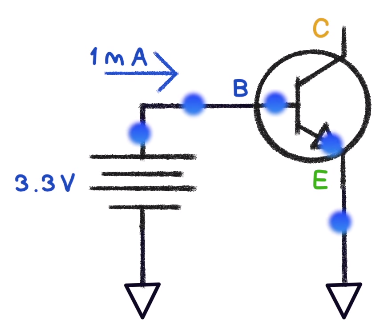
\includegraphics[width=0.3\textwidth]{vbe.png}
\quad
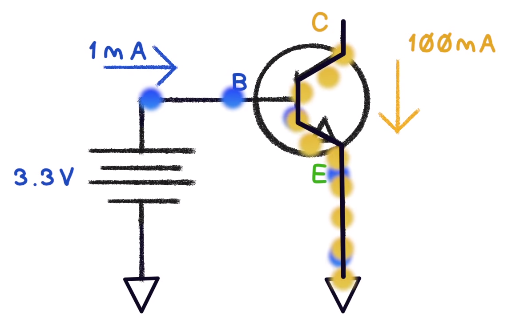
\includegraphics[width=0.4\textwidth]{vce.png}
\end{align*}

The key to this transistor is that 100mA flows from the collector to the emitter. The relationship between these two currents is known as the gain of the transistor. For example, for a 2N3904 BJT, the datasheet states that its gain (also known as $\beta$ or \emph{hFE}) should be 100, varying under different conditions and should be treated as a guideline to follow, whilst not being an absolute rule. Using a simple formula, its possible to calculate the maximum current that the transistor will allow through its collector to its emitter:
$$I_C=I_B*\beta$$
But how do we know what the base current should be? Within a BJT, there is a set of diodes that must be limited in their current in order to work correctly as intended. A standard diode has a forward voltage of about 0.7V. Therefore the current limiting resistor must drop to approximately 2.6V in order to function correctly under Ohm's Law.
$$V_F=3.3V-0.7V=2.6V$$
Using the law, the resistance can be calculated:
$$R=\frac{V_R}{I_B}=\frac{2.6V}{1mA}=2600\Omega$$
\begin{align*}
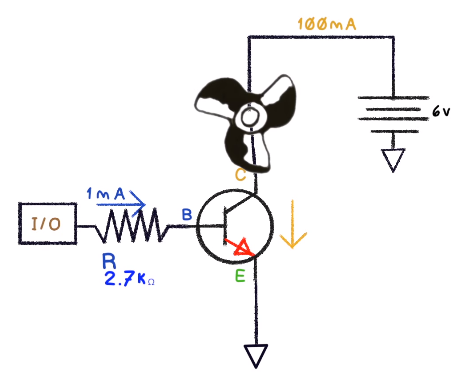
\includegraphics[width=0.4\textwidth]{motor.png}
\end{align*}
This demonstrates two capabilities of the BJT:
\begin{enumerate}
\item It amplifies current by turning 1mA into 100mA
\item It acts as an electronic switch
\end{enumerate}
The above example uses a NPN transistor. A PNP transistor acts similarly, but as seen below, the diodes are inverted and thus behaves in a different manner to that of the NPN transistor, where the arrow on the diagrams point in the direction of the N part of the transistor itself.
\begin{align*}
\centering
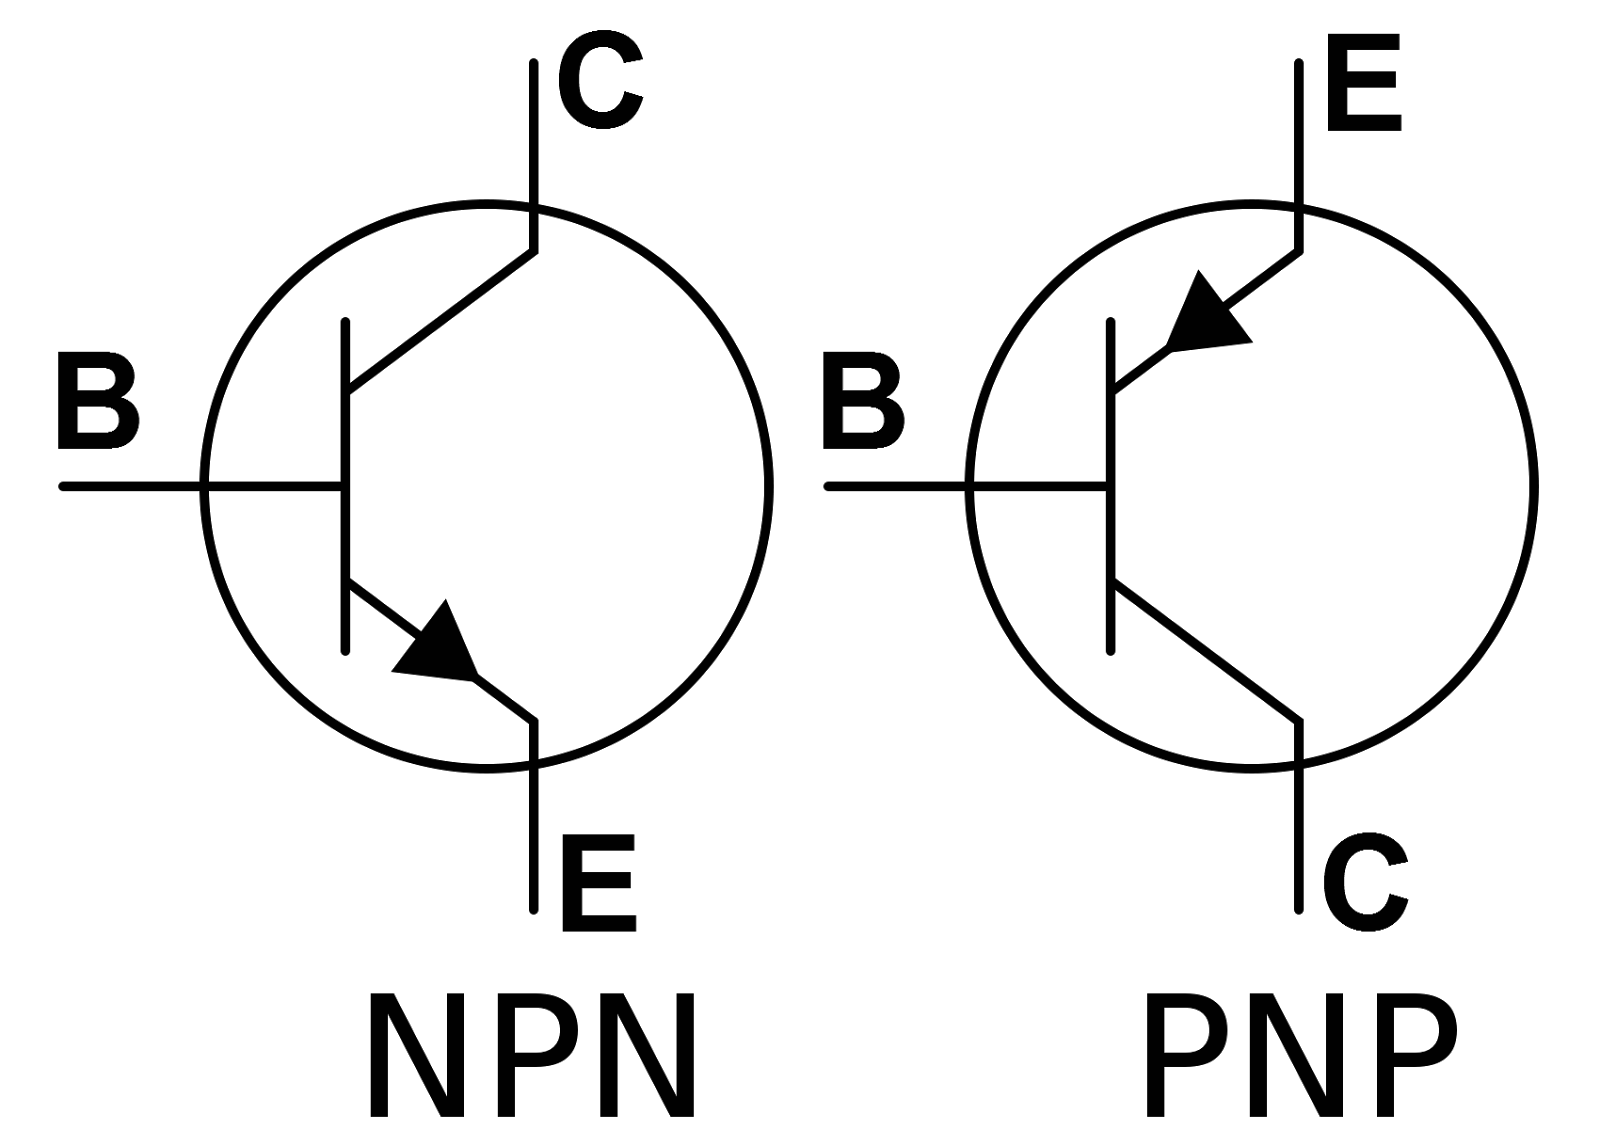
\includegraphics[width=0.3\textwidth]{NPNvsPNP.png}
\end{align*}

\subsubsection{Semiconductor Doping}
Semiconductor doping is the addition of a small percentage of foreign atoms into the regular crystal lattice of silicon or germanium in order to produce dramatic changes in their electrical properties. The addition of doping to a semiconductor creates what is called an N-type or P-type semiconductor, depending on the context of additions.

An impure atom with 5 valence electrons, also called a \emph{pentavalent impurity}, produces an N-type semiconductor by contributing extra electrons that remain in majority.

Impurity atoms with 3 valence electrons, also called a \emph{trivalent impurity}, produces a P-type semiconductor by requiring an electron, and thereby creating a \emph{hole} that must be filled.
\subsubsection{PNP \& NPN}
\subsection{Terminology}
\subsubsection{Applied Electricity}
\begin{itemize}
\item Voltage:
\begin{itemize}
\item Voltage is the different in electric potential energy of a unit charge transported between points a and b.
\end{itemize}
\item Current:
\begin{itemize}
\item Current is the flow of electroms in Coulombs per second (and thus denoted by ampere) past a specific point in an orderly movement electrically.
\end{itemize}
\item Ground:
\begin{itemize}
\item Ground is a reference point for which excess charge may exit the circuit.
\end{itemize}
\item Diode:
\begin{itemize}
\item A diode is a component in electronics that consists of two electronodes: an anode and cathode. It is a semiconductor by its material makeup, and can be used to prevent sudden voltage changes and protects other components.
\end{itemize}
\item Pulse Voltage:
\begin{itemize}
\item Pulse voltage is a burst of energy with a well-defined shape. It consists of having a decay, and may form a pulse train by which the time between each subsequent pulse is a constant pulse interval.
\end{itemize}
\item Switching Speed:
\begin{itemize}
\item Switching speed is the time denoted for the duration of change from state a to state b resulting in a synthesized output that is usable for the specific output requirements.
\end{itemize}
\end{itemize}
\subsubsection{Semiconductor Theory}
\begin{itemize}
\item NPN:
\begin{itemize}
\item NPN transistors have a positive voltage at the base and a negative one at the emitter due to its polarity between the base and the emitter ($V_{BE}$). The collector supply voltage is positive with respect to the emitter ($V_{CE}$). Electrons are the most important carriers for NPN.
\end{itemize}
\item PNP:
\begin{itemize}
\item A PNP transistor is one where polarities are reversed, and its current sinks into its base. This differentiates itself with respect to the NPN transistor by having holes as the most important carrier for the PNP transistor.
\end{itemize}
\item $\beta$:
\begin{itemize}
\item Gain, $\beta$, corresponds to the ratio of change in the signal level between input and output. In the case that $\beta=1$, the net current output has increased by the ratio n.
\end{itemize} 
\item $\beta_f$:
\begin{itemize}
\item This corresponds to the forward-gain of the device in forward active mode. Gain is subject to factors such as temperature and other environmental factors with respect to conditions. $\beta_f$ is approximately equivalent to the ratio of DC collector current to the DC base current in forward active mode of operation. 
\end{itemize}
\item $\beta_r$:
\begin{itemize}
\item The bias conditions subject to reverse active mode correspond to the emitter and collector regions switching roles and causing a significantly smaller $\beta$ than in forward active mode.
\end{itemize}
\item $T_f$:
\begin{itemize}
\item This is the time associated with electronics crossing the transistor junction in forward active mode.
\end{itemize}
\item $T_r$:
\begin{itemize}
\item This is the time associated with electronics crossing the transistor junction in reverse active mode.
\end{itemize}
\item $C_{je}$:
\begin{itemize}
\item $C_{je}$ refers to the equilibrium of system within the base-emitter region of the BJT transistor noted that there is a void of majority charges within this region of operation.
\end{itemize}
\item $C_{jc}$:
\begin{itemize}
\item $C_{jc}$ is referred to as the system's equilibrium pertaining to being void of all majority charges within the base-collector region of operation.
\end{itemize}
\item $V_{be}$:
\begin{itemize}
\item This is the voltage associated with the base-emitter region of operation within the transistor, which is generally used to find a transistor's DC values and thresholds. Its value depends greatly on the material, ie $V_{be}\approx0.7V$ for Silicon, while for Germanium $V_{be}\approx0.3V$
\end{itemize}
\item $V_{be cut-in}$:
\begin{itemize}
\item This value corresponds to when the voltage becomes significant enough to cause an excitation and impulse response within the component. The voltage measured before this value implies that the current supplied is insignificant to the circuit and causes no effect.
\end{itemize}
\item $V_{be sat}$:
\begin{itemize}
\item This value resides on the opposite spectrum to $V_{be cut-in}$. It is the region reached when $V_{be}$ becomes greater than 0.7V. Applying a greater voltage beyond this point may cause an adverse effect of exponential scaling, thus leading to an extremely high current through the transistor.
\end{itemize}
\item $V_{ce}$:
\begin{itemize}
\item This is the voltage that resides in the collector-emitter region of a bipolar junction transistor.
\end{itemize}
\item $V_{ol}$:
\begin{itemize}
\item This is the maximum value of voltage needed in order to return a digital 0 in logic residing below the indeterminate buffer zone where the level is neither 0 nor 1.
\end{itemize}
\item $V_{oh}$:
\begin{itemize}
\item This is the minimum value of voltage needed in order to return a digital 1 in logic, residing above the indeterminate buffer zone of undefined logic.
\end{itemize}
\item $V_{il max}$:
\begin{itemize}
\item This is the maximum input voltage required in order to recognise a logical 0.
\end{itemize}
\item $V_{ih min}$:
\begin{itemize}
\item This is the minimum input voltage required in order to recognise a logical 1.
\end{itemize}
\item Signal swing:
\begin{itemize}
\item The quantity by which a signal changes, ie a measure of its amplitude change over a period of time.
\end{itemize}
\end{itemize}

\section{Current vs Base-Emitter Voltages}
\subsection{Method}
\begin{enumerate}
\item Following instructions in the schematic entry given in the lab book, set the circuit up as the following diagram
\begin{align*}
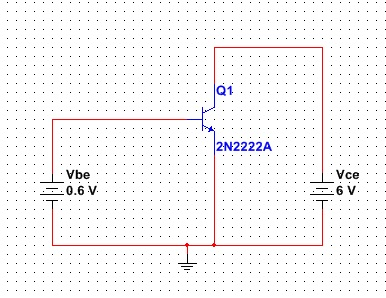
\includegraphics[width=0.4\textwidth]{a1_circuit.jpg}
\end{align*}
\item Using component properties, the following table is to be filled in
\end{enumerate}
\begin{table}[h]
\centering
\begin{tabular}{ll}
$\beta_f$  & 220  \\
$\beta_r$  & 4 \\
$\tau_f$  & $0.325x10^{-9}s$      \\
$\tau_r$  & $100x10^{-9}s$        \\
$C_{jc}$ & $9.12x10^{-12}F$        \\
$C_{je}$ & $2.701x10^{-11}F$        
\end{tabular}
\caption{Recorded values for 2N2222A}
\end{table}
\subsection{Simulation}
In  simulation for this, a DC Sweep is used and the output is interpreted as a curved graph with respect to the following specifications for $V_{BE}$, noting that source two is not in use:
\begin{table}[h]
\centering
\begin{tabular}{ll}
Start value 	& 	0.2V  \\
Stop value  	& 	0.9V   \\
Increments  	&   0.01V 
\end{tabular}
\caption{A1 DC Sweep Values}
\end{table}
Also note that $I(V_{CE})$ must be inverted by multiplying by -1 under the configuration settings.
\subsection{Results}
\begin{align*}
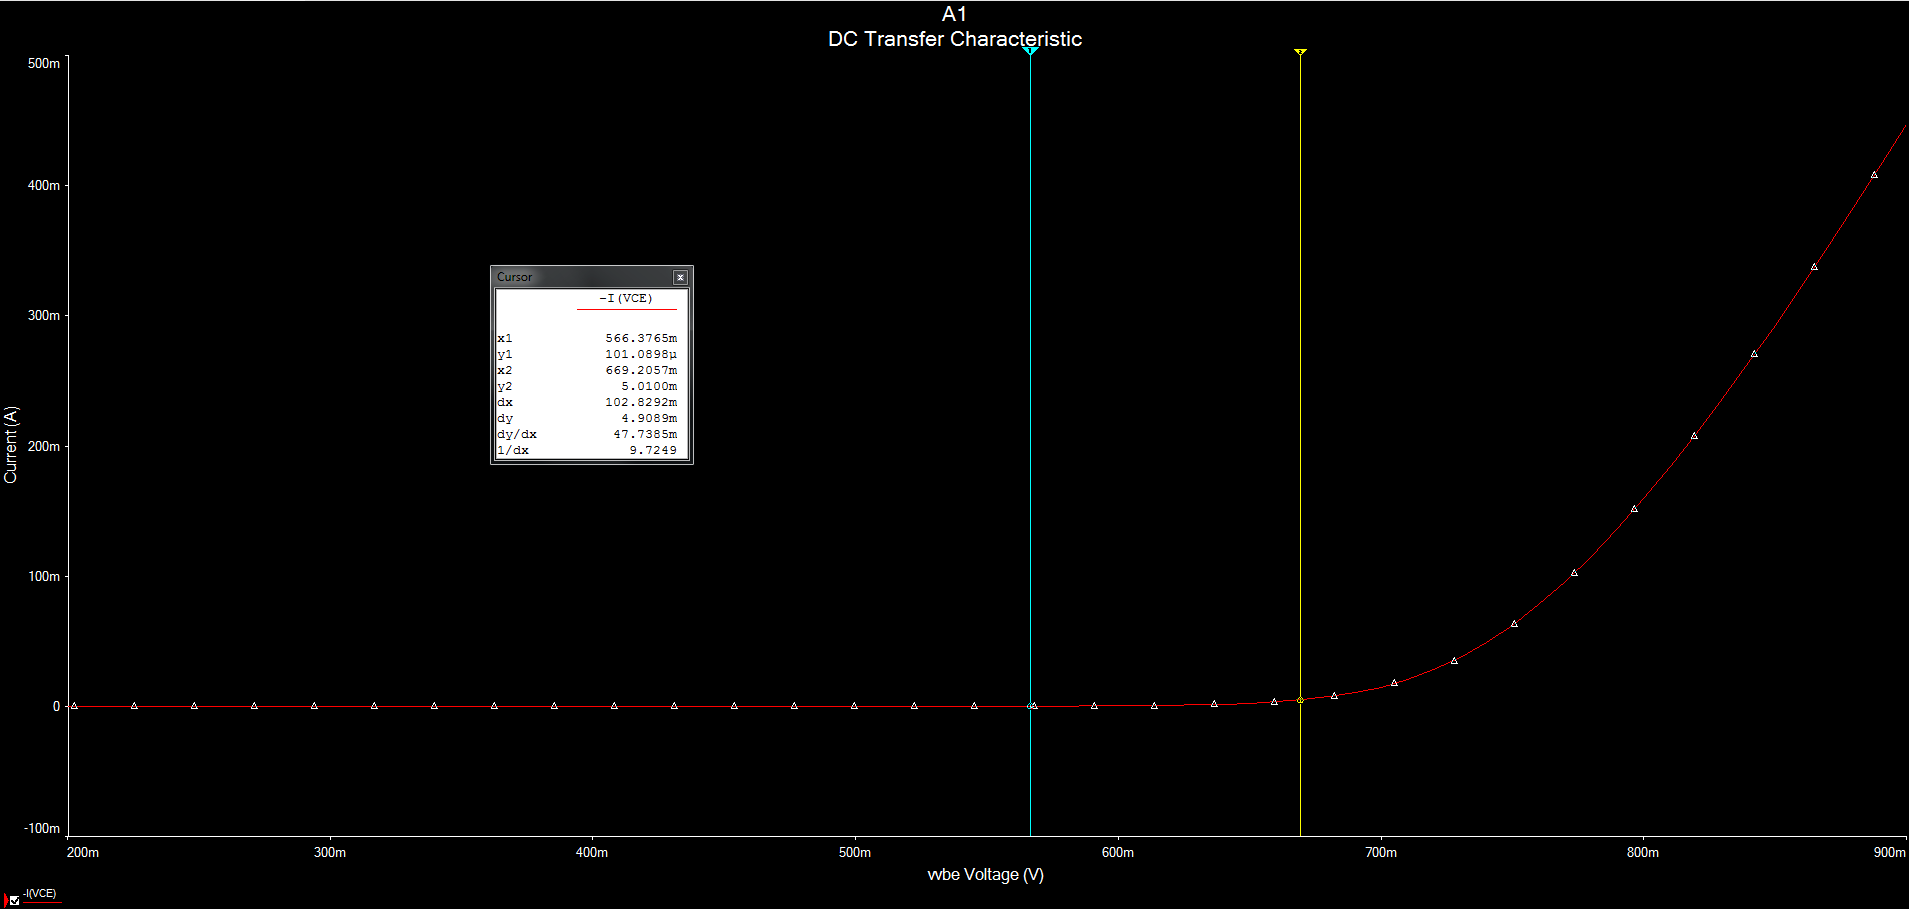
\includegraphics[width=1\textwidth]{A1.png}
\end{align*}
\begin{table}[h]
\centering
\begin{tabular}{ll}
$V_{be cut-in}$  & 0.566V  \\
$V_{be on}$  & 0.669V      
\end{tabular}
\caption{Recorded values for voltages}
\end{table}
In comparison to the lectures, my results are approximately the same as the figures given, therefore they are within a reasonable range of accuracy.

\section{Collector Current vs Collector-Emitter Voltage}
\subsection{Method}
\begin{enumerate}
\item Following instructions in the schematic entry given in the lab book, set the circuit up as the following diagram
\end{enumerate}
\begin{align*}
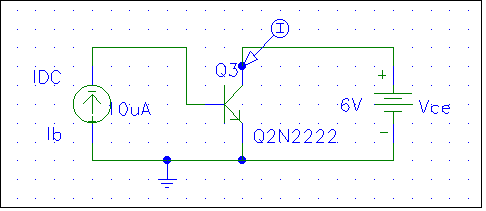
\includegraphics[width=0.6\textwidth]{a2_circuit.png}
\end{align*}
\subsection{Simulation}
Again as before, a  DC Sweep is performed on the circuit to the following specifications:
\begin{table}[h]
\centering
\begin{tabular}{ll}
$V_{CE}$			&	\\
Start value		&$0V$\\
Stop value		&$6V$\\
Increment		&$0.05V$\\
$I_{B}$			&\\
Start value		&$1e-005AV$\\
Stop value		&$0.0001A$\\
Increment		&$1e-005A$
\end{tabular}
\caption{DC sweep parameters for analysis}
\end{table}
\subsection{Results}
Using the following formula, $I_C=\beta_FI_B$, the forward gain ($\beta_F$) can be found for various values.
\begin{table}[h]
\centering
\begin{tabular}{ll}
$\beta_{F} @ I_{B} = 10 \mu A$ & 210 \\
$\beta_{F} @ I_{B} = 100 \mu A$ & 217 \\
$V_{ce sat}@I_{C}\approx5mA $ & 0.211V
\end{tabular}
\caption{Recorded voltages  2N2222 for collector-emitter}
\end{table}
\begin{table}[h]
\centering
\begin{tabular}{ll}
$\beta_{F} @ I_{B} = 10 \mu A$ & 142 \\
$\beta_{F} @ I_{B} = 100 \mu A$ & 131 \\
$V_{ce sat}@I_{C}\approx5mA $ & 0.188V
\end{tabular}
\caption{Recorded voltages 2N3904 for collector-emitter}
\end{table}

\section{Resistively Loaded Transfer Characteristics}
\subsection{Method}
\begin{enumerate}
\item Set up an entirely new circuit with respect to the diagram below.
\item Ensure that a pulse voltage is used on the base-emitter with a 2N2222A BJT, and another power source on the collector-emitter side.
\item Two resistors should be in their given places with their respective resistance.
\end{enumerate}
\begin{align*}
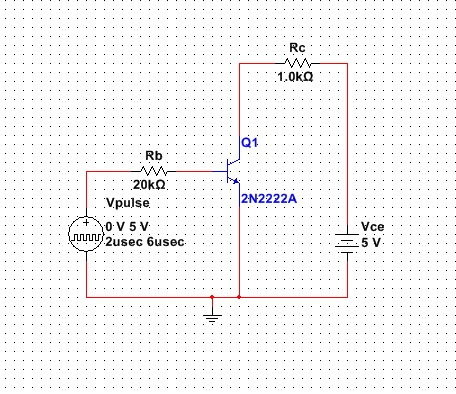
\includegraphics[width=0.6\textwidth]{b_circuit.jpg}
\end{align*}
\subsection{Simulation}
In accordance to the image below, pulse voltage is set up as such, where any other values are to be set to 0.
\begin{table}[h]
\centering
\begin{tabular}{ll}
Initial value & $0V$ \\
Pulsed value & $5V$ \\
Delay time & $1 \mu s$ \\
Rise itme & $0 s$ \\
Fall time & $0 s$ \\
Pulse width & $2 \mu s$ \\
Period & $6 \mu s$
\end{tabular}
\caption{Pulse voltage parameters}
\end{table}
A DC sweep is performed such that the following analysis parameters are obeyed with the specific variables selected for analysis:
\begin{table}[h]
\centering
\begin{tabular}{ll}
Start value & $0V$ \\
Stop value & $5V$ \\
Increment & $0.01V$
\end{tabular}
\caption{DC sweep parameters}
\end{table}
\subsection{Results}
\begin{align*}
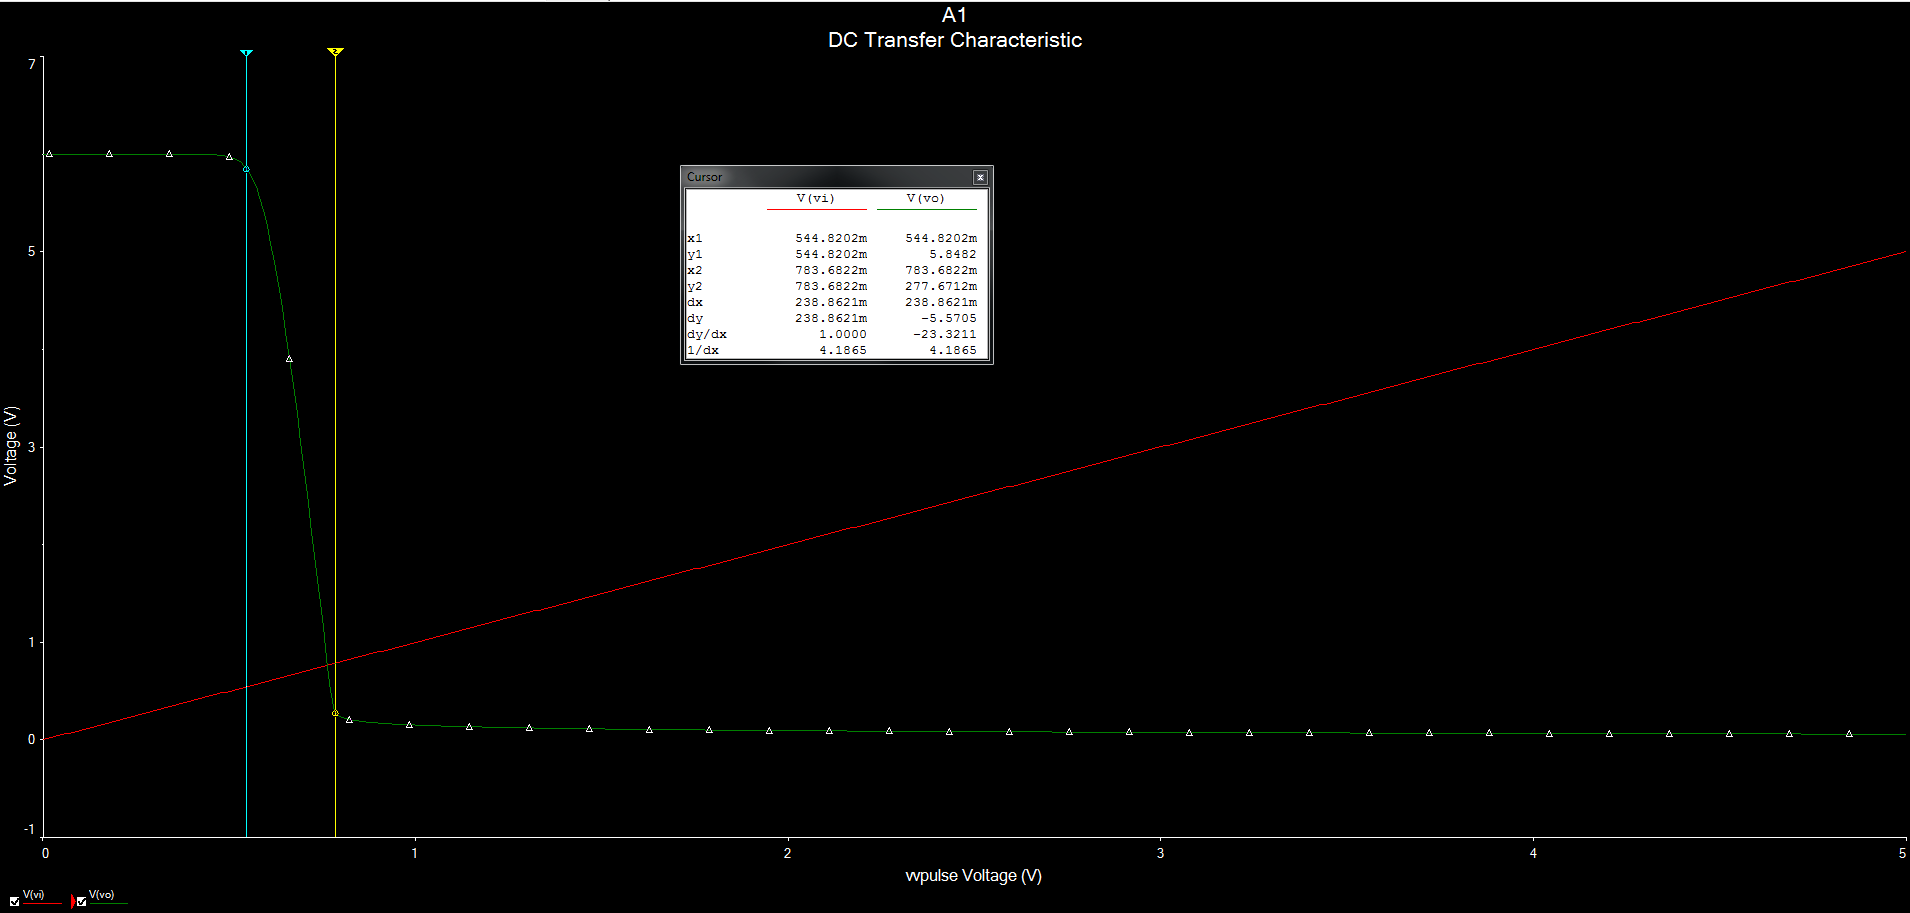
\includegraphics[width=1\textwidth]{b1ii.PNG}
\end{align*}
\begin{table}[h]
\centering
\begin{tabular}{ll}
$V_{OH}$ 		& 5.88V \\
$V_{IL max}$ 	& 0.582V \\
$V_{OL}$ 		& 0.319V \\
$V_{IH min}$ 	& 1.232V
\end{tabular}
\caption{Recorded voltages for a resistively loaded BJT}
\end{table}
\begin{table}[h]
\centering
\begin{tabular}{ll}
$V_{OH}=V_{CC}=$ & 5V\\
$V_{OL}=V_{CE sat}=$ & 0.3V\\
$V_{IL max}=V_{VE cut-in}$ & 0.6V\\
$V_{IH min}=V_{BE on} + \frac{R_{b}}{\beta_{f}R_{c}}\left[V_{CC}-V_{CE sat}\right]$ & 1.2V
\end{tabular}
\caption{Theory v Measured Values}
\end{table}
\section{Switching Characteristics}
\subsection{Method}
Reuse the circuit from B and ensure that the transient analyses have been set up appropriately to the following specifications:
\begin{table}[h]
\centering
\begin{tabular}{ll}
Initial conditions	&	Determine automatically\\
Start time			&	$0s$\\
End time				&	$6e-006s$\\
Maximum step time	&	$1e-008s$
\end{tabular}
\caption{Transient analysis}
\end{table}
\subsection{Simulation}
Align the cursors to the appropriate areas of the graph as shown in order to retrieve the appropriate values for each section:
\begin{align*}
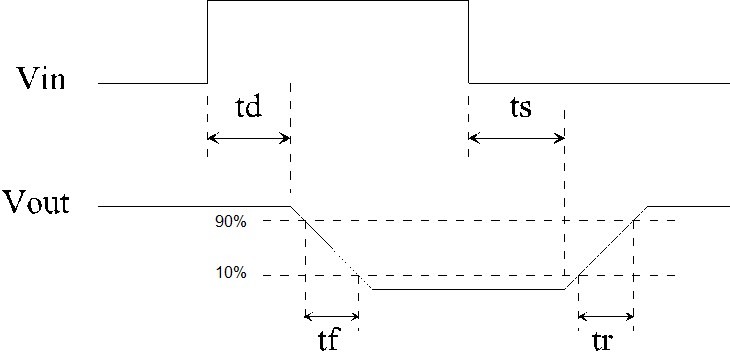
\includegraphics[width=0.5\textwidth]{c_times.png}
\end{align*}
\subsection{Results}
The following are the resulting graphs for $R_b=20k\Omega$, $R_{b}=5k\Omega$, and $R_{c}=4k\Omega$; noting the change in slopes for each subsequent value.
\begin{align*}
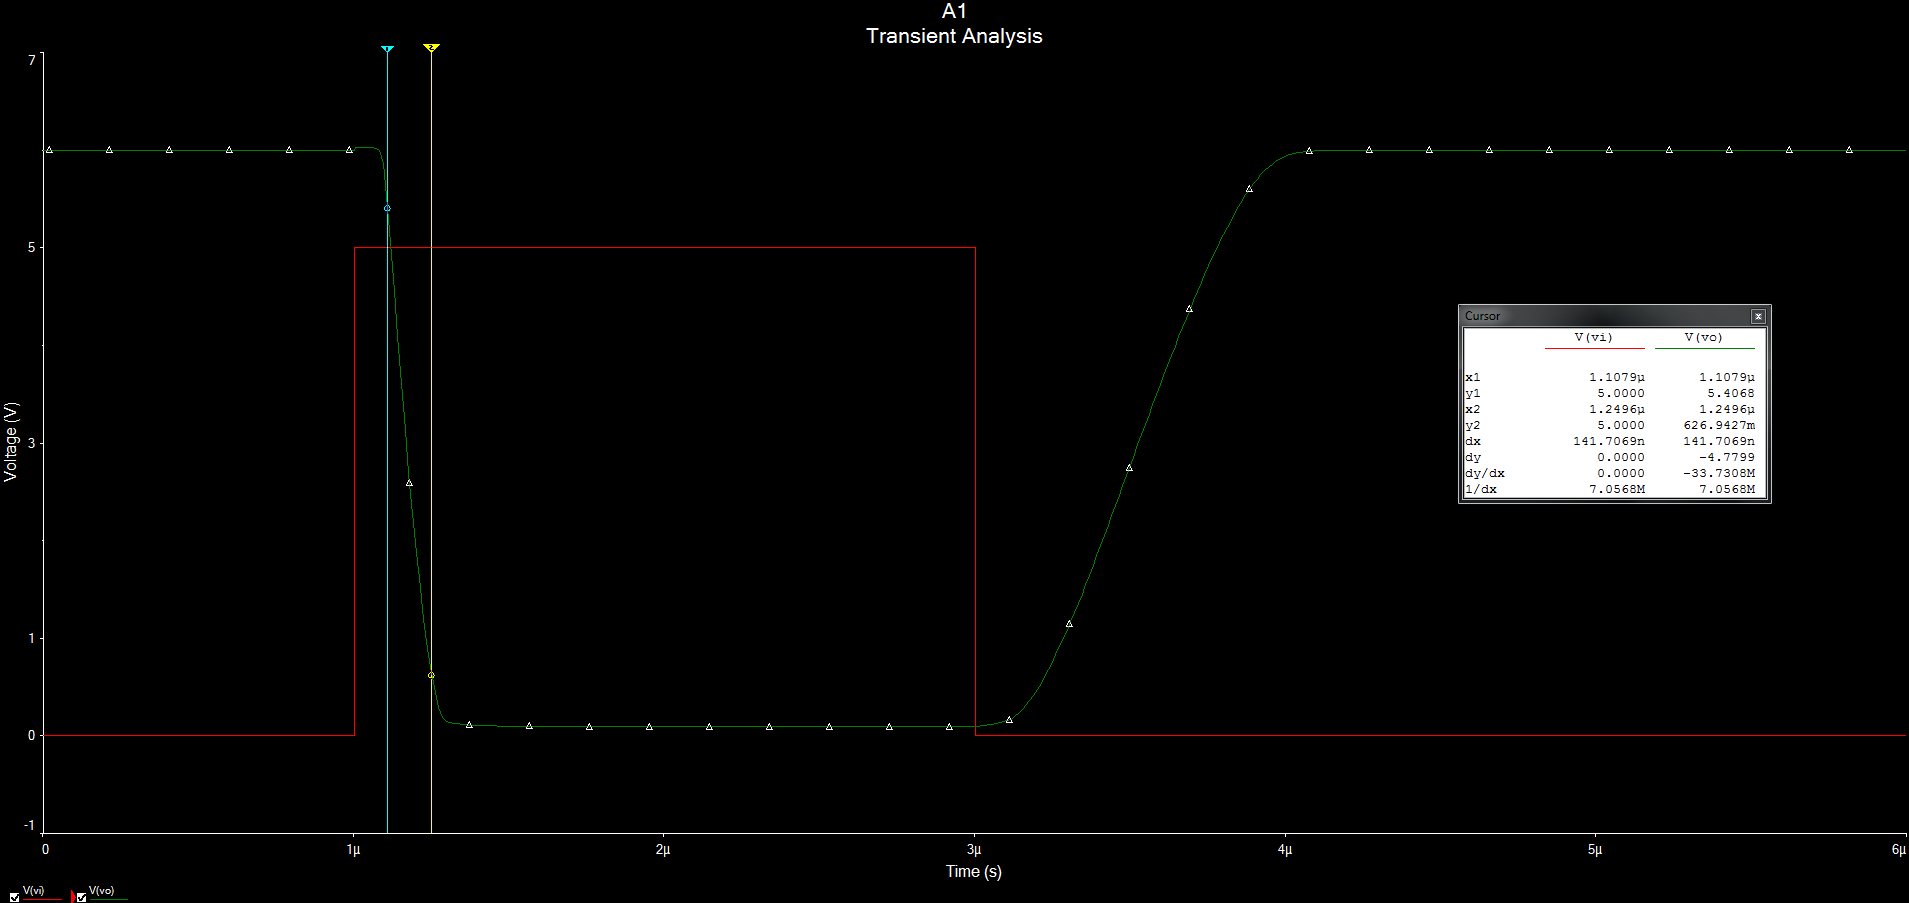
\includegraphics[width=0.75\textwidth]{c1.PNG}
\end{align*}
\begin{align*}
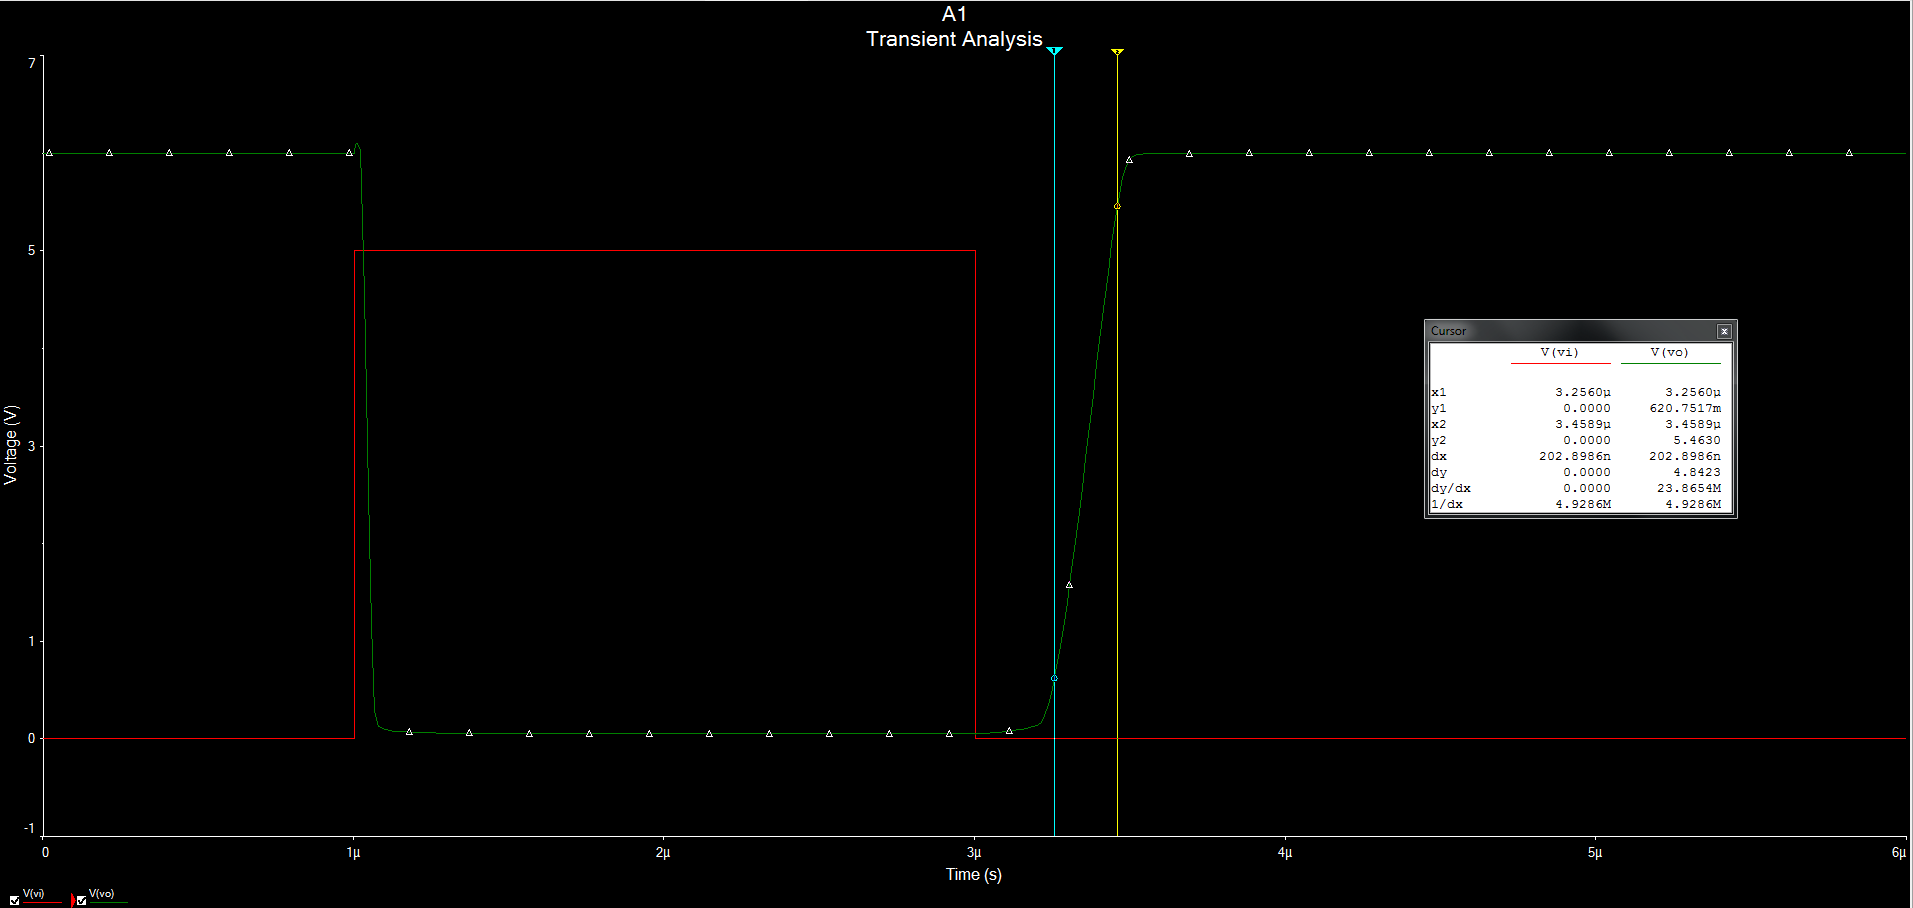
\includegraphics[width=0.75\textwidth]{c2.PNG}
\end{align*}
\begin{align*}
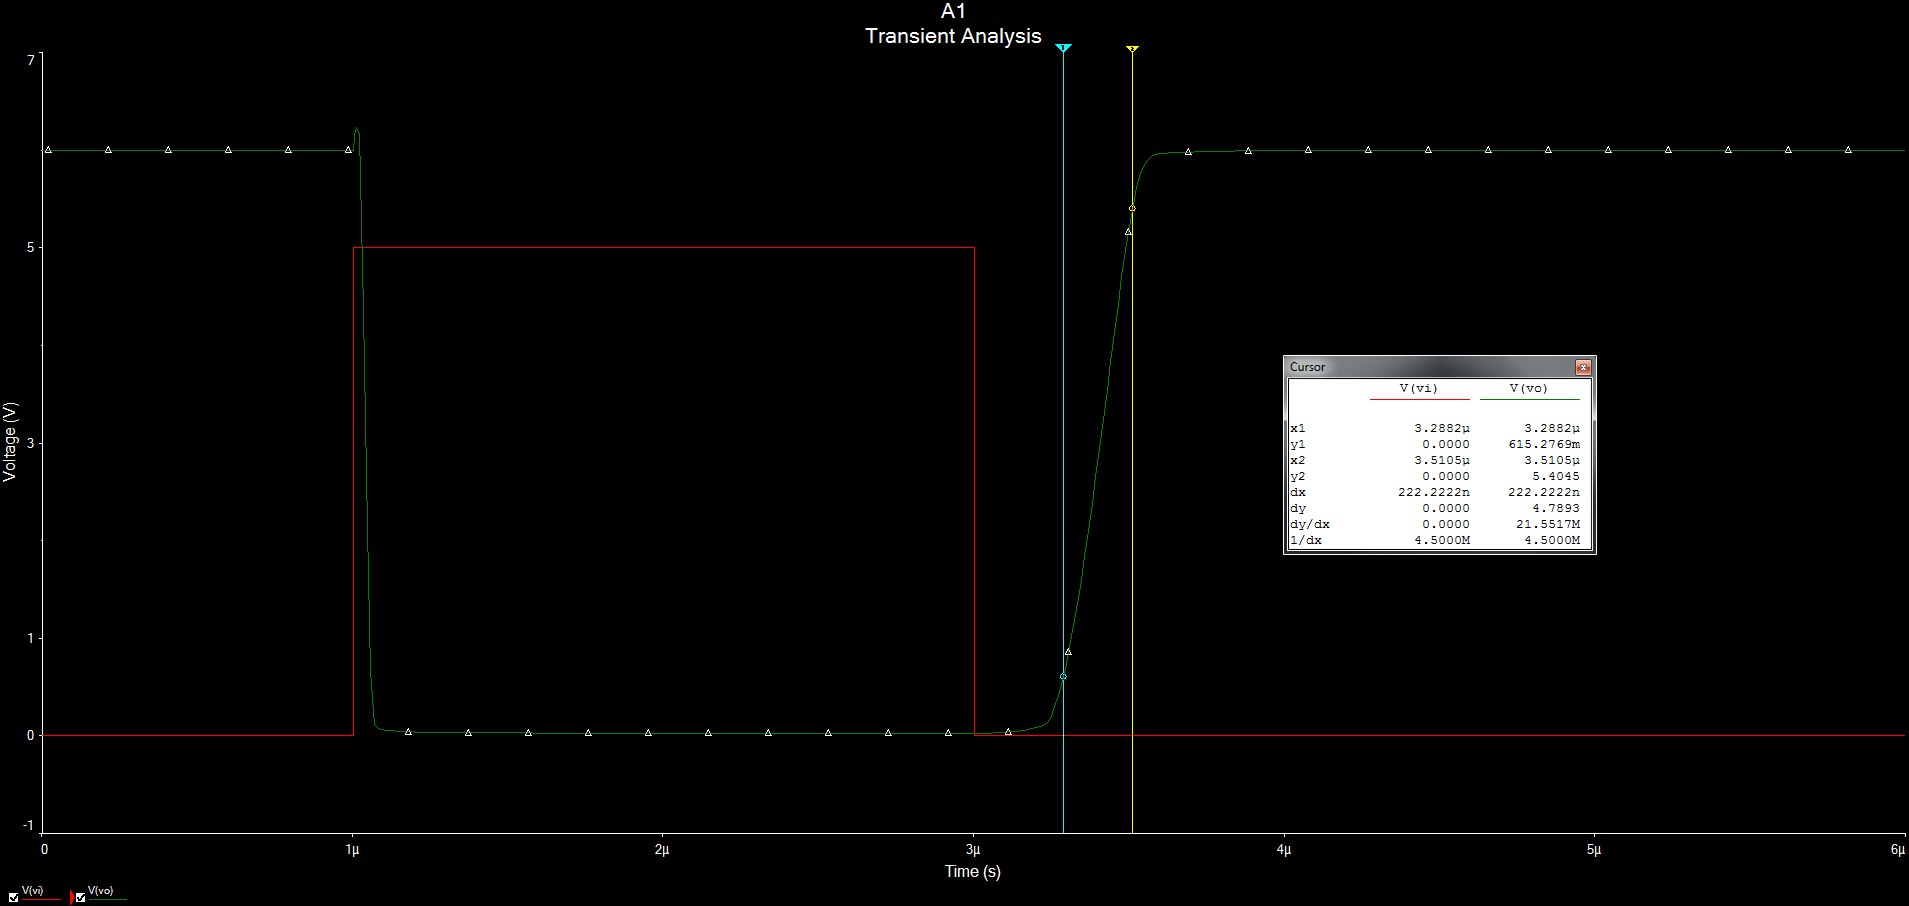
\includegraphics[width=0.75\textwidth]{c3.PNG}
\end{align*}
\begin{table}[h]
\centering
\begin{tabular}{ll}
$t_d$ & $0.1417\mu s$\\
$t_f$ & $0.1256\mu s$\\
$t_s$ & $0.1256\mu s$\\
$t_r$ & $0.6216\mu s$
\end{tabular}
\caption{Theory v Measured Values}
\end{table}
Following on values obtained from A1:
%via values from A1
$$t_d=R_b\left(C_{je}+C_{jc}\right)In\left[\frac{V_{CC}}{V_{CC}-V_{BE cut-in}}\right]=8.746x10^{-8}s$$
$$t_f=0.8\beta_F\left(\tau_F+R_cC_{jc}\right)In\left[\frac{\beta_FI_{BF}}{\beta_FI_{BF}-I_{C max}}\right]=1.418x10^{-7}s$$
$$t_s=\tau_sIn\left[\frac{I_{BF}-I_{BR}}{\frac{I_{C max}}{\beta_F}-I_{BR}}\right]=1.351x10^{-7}s$$
$$t_r=0.8\beta_F\left(\tau_F+R_CC_{jc}\right)In\left[\frac{\frac{I_C max}{\beta_F}-I_{BR}}{-I_{BR}}\right]=1.239x10^{-6}s$$
where
$$I_{BF}=\frac{V_I-V_{BE on}}{R_b}=2.658x10^-4A$$
$$I_{C max}=\frac{V_{CC}-V_{CE on}}{R_C}=4.936x10^{-3}A$$
$$I_{BR}=-\frac{V_{BE on}}{R_B}=-5.7x10^{-4}A$$
$$\tau_s=\frac{(1-\beta_R)\tau_{BF}+\beta_F\tau_{BR}}{1+\beta_F+\beta_R}=\frac{(1+\beta_R)\beta_F\tau_F+\beta_R\beta_F\tau_R}{1+\beta_F+\beta_R}=3.927x10^-{-7}s$$
\begin{table}[!h]
\centering
\begin{tabular}{ll}
$t_d$ & $8.746x10^{-8}s$\\
$t_f$ & $1.418x10^{-7}s$\\
$t_s$ & $1.351x10^{-7}s$\\
$t_r$ & $1.239x10^{-6}s$
\end{tabular}
\caption{Theory v Measured Values from equations}
\end{table}
\begin{table}[!h]
\centering
\begin{tabular}{ll}
$t_d$ & $0.02\mu s$\\
$t_f$ & $0.036\mu s$\\
$t_s$ & $0.26\mu s$\\
$t_r$ & $0.2\mu s$
\end{tabular}
\caption{Measured Values of $R_b$ to $5k\Omega$}
\end{table}
\begin{table}[!h]
\centering
\begin{tabular}{ll}
$t_d$ & $0.01\mu s$\\
$t_f$ & $0.032\mu s$\\
$t_s$ & $0.23\mu s$\\
$t_r$ & $0.222\mu s$
\end{tabular}
\caption{Measured Values of $R_c$ to $4k\Omega$}
\end{table}

\section{Discussion}
\begin{itemize}
\item A1 - Collector Current against Base-Emitter Voltage
\begin{itemize}
\item How do the values of $V_{be cut in}$ and $V_{be on}$ compare with those in lectures?
\begin{itemize}
\item Saturation occurs when the Base-Emitter region reaches a maximum under conditions of bias having been reached. Therefore, as current increases with voltage, at this point, the voltage will be higher than that of $V_{be on}$. With respect to lectures, the values are within range of reasonable tolerance.
\end{itemize}
\end{itemize}
\item B - Resistively Loaded BJT Inverter Transfer Characteristics
\begin{itemize}
\item Compare these measurements with calculations from theory and previous device measurements.
\begin{itemize}
\item $V_{OH}=V_{CC}=5.88V-5V=0.88V$ difference
\item $V_{OL}=V_{CE sat}=0.319V-0.3V=0.019V$ difference
\item $V_{IL max}=V_{BE cut in}=0.6V-0.582V=0.018V$ difference
\item $V_{IH min}=V_{BE on} + \frac{R_{b}}{\beta_{f}R_{c}}\left[V_{CC}-V_{CE sat}\right]=1.232V-1.2V=0.032V$ difference
\end{itemize}
\item Predict what will happen is $R_C$ is increased from $1k\Omega$ to $4k\Omega$.
\begin{itemize}
\item Reducing $R_b$ causes the slops of the graph of the input vs output voltage to increase and therefore causes an increase in $V_{OL}$.
\end{itemize}
\end{itemize}
\item C - BJT Inverter - Switching Characteristics
\begin{itemize}
\item Predict what will happen is $R_B$ is reduced to $5k\Omega$.
\begin{itemize}
\item Increasing $R_c$ does the opposite of increasing $R_b$, and therefore increases $V_{OL}$.
\end{itemize}
\item Predict what will happen is $R_C$ is increased to $4k\Omega$.
\begin{itemize}
\item Increasing $R_c$ does the opposite of increasing $R_b$ and therefore increases the slope and lowers $V_{OL}$.
\end{itemize}
\end{itemize}
\item Sources of error
\begin{itemize}
\item As my results are not entirely equivalent to results shown in the lecture notes, they have a certain degree of error in them due to approximations and eyeballing.
\item Slopes from the graphs were over a range of tiered edges, and so rather than viewing a single point at which change started, I had to approximate the point at which enough change had happened in order to deem it as entering a new stage of voltage.
\end{itemize}
\end{itemize}
\section{Conclusion}
\subsection{Findings}
Overall my results were approximately close to the actual values within the lecture notes. On comparison to values that one would expect to find for such circuitry, my results, albeit with slight error, were within a reasonable tolerance and weren't far from actual values that an electronic engineer would expect to find in a non-ideal environmental situation.
\subsection{Issues for Consideration}
\begin{enumerate}
  \item \textbf{What are the limitations on the accuracy of your results?} \hfill \\
  MultiSim is a development environment that does not take in environmental factors into account, therefore the values acquired here are absolute under perfect circumstances. In real life, the actual values may differ due to slight differences in manufacture per component, environmental temperature, and so forth.
  \item \textbf{How do the values of parameters measured compare with those obtained in lectures?} \hfill \\
  Human error and rounding results may result in values that are only approximately equivalent to those found in the lecture notes. Therefore it is possible that my results are slightly inaccurate due to discrepancies in knowing what point on a curve to take, even if the result was in a simulated, perfect environment.
  \item \textbf{What are the advantages or disadvantages of circuit simulations such as those carried out in the experiments?} \hfill \\
  The values obtained within the lab were quite similar to those found within the lecture notes. As a general finding, the values found within the lecture slides tended to be more rounded, rather than those obtained in the lab which entailed a larger range of decimals.
  \item \textbf{What are the benefits or drawbacks of circuit simulation and of MultiSim in general as applied ot the design of electronic circuits?} \hfill
  \begin{itemize}
  \item Within the time slot provided, it was a benefit that I was able to create and test a series of 3 circuits in the space of a 3 hour slot. If I were to manually assemble these and test using apparatus from the laboratory, it would have taken substantially longer time intervals than that in a simulated environment.
  \item As a general rule of thumb, it was a drawback that this was entirely simulated and does not adhere to real-world conditions such as non-ideal temperature, wear, and other non-ideal factors that aren't accounted for in the perfect world.
  \end{itemize}
  \item \textbf{What are the essential elements of good circuit simulation and simulators?} \hfill
  \begin{itemize}
  \item A good circuit simulation is one that effectively tests the circuit to allow the circuit to function as intended in real life without worrying about malfunction.
  \item A good circuit simulator offers a user-friendly UI that allows the user to work effectively and efficiently with the task at hand with a large library of readily-available functions and components for use within the simulation with respect to the current technology available.
  \end{itemize}
  \item \textbf{What is the role of the Electronic Engineer in this regard?} \hfill \\
  The electronic engineer must understand a deep level of circuitry in order to accurately build a circuit that functions as required. This also entails a lot of testing such that, within an environment such as MultiSim, that everything works as intended and limits are observed.
\end{enumerate}
\section{Bibliography}
\begin{thebibliography}{3}
\bibitem{streetmanb}
  Ben G. Streetman \& Sanjay Kumar Banerjee,
  \emph{Solid State Electronic Devices, 6th edition},
  Prentice Hall (2006),
  Pages 154-388.
\bibitem{sedraa}
Adel S. Sedra \& Kenneth C. Smith,
  \emph{Microelectronic Circuits, 2nd edition},
  Oxford University Press (1987).
\bibitem{horowitzp}
Paul Horowitz \& Winfield Hill
  \emph{The Art of Electronics, 2nd edition},
  Cambridge University Press (1989).
\end{thebibliography}
\end{document}
